\documentclass[coursework]{SCWorks}
% Тип обучения (одно из значений):
%    bachelor   - бакалавриат (по умолчанию)
%    spec       - специальность
%    master     - магистратура
% Форма обучения (одно из значений):
%    och        - очное (по умолчанию)
%    zaoch      - заочное
% Тип работы (одно из значений):
%    coursework - курсовая работа (по умолчанию)
%    referat    - реферат
%  * otchet     - универсальный отчет
%  * nirjournal - журнал НИР
%  * digital    - итоговая работа для цифровой кафедры
%    diploma    - дипломная работа
%    pract      - отчет о научно-исследовательской работе
%    autoref    - автореферат выпускной работы
%    assignment - задание на выпускную квалификационную работу
%    review     - отзыв руководителя
%    critique   - рецензия на выпускную работу

% * Добавлены вручную. За вопросами к @mchernigin
\usepackage{preamble}

\begin{document}

% Кафедра (в родительном падеже)
\chair{математической кибернетики и компьютерных наук}

% Тема работы
\title{Разработка ядра клиент-серверного приложения для "Отработки" для андроида}

% Курс
\course{2}

% Группа
\group{251}

% Факультет (в родительном падеже) (по умолчанию "факультета КНиИТ")
% \department{факультета КНиИТ}

\napravlenie{09.03.04 "--- Программная инженерия}

% Для студентки. Для работы студента следующая команда не нужна.
% \studenttitle{студентки}

% Фамилия, имя, отчество в родительном падеже
\author{Смирнова Егора Ильича}

% Заведующий кафедрой 
\chtitle{доцент, к.\,ф.-м.\,н.}
\chname{С.\,В.\,Миронов}

% Руководитель ДПП ПП для цифровой кафедры (перекрывает заведующего кафедры)
% \chpretitle{
%     заведующий кафедрой математических основ информатики и олимпиадного\\
%     программирования на базе МАОУ <<Ф"=Т лицей №1>>
% }
% \chtitle{г. Саратов, к.\,ф.-м.\,н., доцент}
% \chname{Кондратова\, Ю.\,Н.}

% Научный руководитель (для реферата преподаватель проверяющий работу)
\satitle{доцент, к.\,ф.-м.\,н.} %должность, степень, звание
\saname{И.\,А.\,Батраева}

% Руководитель практики от организации (руководитель для цифровой кафедры)
% \patitle{доцент, к.\,ф.-м.\,н.}
% \paname{С.\,В.\,Миронов}

% Руководитель НИР
% \nirtitle{доцент, к.\,п.\,н.} % степень, звание
% \nirname{В.\,А.\,Векслер}

% Семестр (только для практики, для остальных типов работ не используется)
\term{2}

% Наименование практики (только для практики, для остальных типов работ не
% используется)
% \practtype{учебная}

% Продолжительность практики (количество недель) (только для практики, для
% остальных типов работ не используется)
% \duration{2}

% Даты начала и окончания практики (только для практики, для остальных типов
% работ не используется)
% \practStart{01.07.2024}
% \practFinish{13.01.2024}

% Год выполнения отчета
\date{2025}

\maketitle

% Включение нумерации рисунков, формул и таблиц по разделам (по умолчанию -
% нумерация сквозная) (допускается оба вида нумерации)
% \secNumbering

\tableofcontents

% Раздел "Обозначения и сокращения". Может отсутствовать в работе
% \abbreviations
% \begin{description}
%     \item ... "--- ...
%     \item ... "--- ...
% \end{description}

% Раздел "Определения". Может отсутствовать в работе
% \definitions

% Раздел "Определения, обозначения и сокращения". Может отсутствовать в работе.
% Если присутствует, то заменяет собой разделы "Обозначения и сокращения" и
% "Определения"
% \defabbr

\intro
Цель работы --- разработка серверной части системы для приложения "Отработки" с REST API на .NET.

Задачи работы:
\begin{itemize}
	\item{Изучить принципы разработки серверных приложений на .NET.}
	\item{Спроектировать архитектуру серверной части.}
	\item{Реализовать API для управления пользовтелями, запросами на отработку.}
\end{itemize}

% После введения — серии \section, \subsection и т.д.

\section{Теоритеческая часть}
\subsection{Клиент"=серверная архитектура}

В современных информационных системах эффективное взаимодействие между различными приложениями и сервисами является ключевым фактором успешной реализации бизнес-логики и обеспечения высокого уровня обслуживания пользователей. Одним из наиболее распространённых и универсальных подходов к организации такого взаимодействия является использование REST API.

Передача представления состояния (Representational State Transfer, сокращенно REST) --- это стиль архитектуры, для проектирования сетевых приложений. REST API основан на модели связи клиент"=сервер, где клиент с помощью HTTP"=запросов на сервер получает информацию в формате JSON, XML, HTML и так далее. Вся информация на сервере представлена в виде ресурсов и подресурсов: пользователи приложения, загруженные файлы и прочее. У каждого ресурса есть свой уникальный идентификатор, ресурс имеет состояние, и клиент может получать или изменять состояние ресурса при помощи представлений (как уже упоминалось ранее, под представлением можно понимать JSON, XML, текст в определённом формате или что угодно, что позволяет нам понимать текущее состояние ресурса). При этом серверная часть никак не зависит от клиентской, клиентом веб"=сервиса может выступать браузер пользователя, мобильное приложение, другой сервер и так далее.

В REST для манипулирования ресурсами используются стандартные HTTP"=методы:
\begin{itemize}
	\item{GET --- получение содержимого;}
	\item{POST --- создание содержимого;}
	\item{PUT --- обновление содержимого;}
	\item{DELETE --- удаление содержимого;}
\end{itemize}

Запросы в такой архитектуре являются самодостаточными, серверу при их обработке нет необходимости извлекать контекст приложения, поскольку клиент включает в запрос все необходимые данные, использую для этого заголовки и тело запроса. Такой подход повышает производительность, упрощает дизайн и реализацию серверных компонентов системы.

Для REST API выделяются несколько основных принципов:
\begin{enumerate}
	\item{использование клиент"=серверной модели связи;}
	\item{использование стандартных HTTP"=методов;}
	\item{использование уникальных идентификаторов ресурсов;}
	\item{работа с данными через представления в формате JSON;}
	\item{отсутствие состояния на стороне сервера;}
\end{enumerate}

Соблюдение перечисленных принципов повышает надёжность и производительность приложения.

\subsection{Технологии backend-разработки на .NET}

\subsubsection{ASP.NET Core: Особенности, middleware}

\subsubsection{Оптимизация работы с бд: репозитории}

\subsection{Безопасность веб"=приложения}

В свете растущих угроз безопасности веб-сервисов особое внимание уделяется надёжным механизмам защиты пользовательских данных. Ключевыми элементами такой защиты являются процессы аутентификации и авторизации, обеспечивающие контроль доступа к ресурсам, а также безопасное хранение паролей с использованием современных методов хэширования. Рассмотрение этих аспектов позволит минимизировать риски несанкционированного доступа и защитить пользователей от компрометации их учётных записей.

\subsubsection{Аутентификация и авторизация (JWT)}

% NOTE: Подводка к JWT
Аутентификация и авторизация --- это фундаментальные компоненты безопасности любой информационной системы, особенно актуальные в области веб"=приложений и сервисов. Они играют решающую роль в защите конфиденциальности и целостности данных, а также в обеспечении контроля доступа к ресурсам и функциям системы.\cite{jwt1}

Аутентификация --- это процесс проверки личности пользователя или устройства, который запрашивает доступ к защищенным ресурсам. Этот процесс включает в себя проверку различных учетных данных, таких как:
\begin{itemize}
	\item{Почта и пароль пользователя: самый распространенный метод аутентификации, который используется для входа в систему.}
	\item{Биометрические данные: распознавание лиц и другие уникальные физиологические характеристики}
	\item{Одноразовые пароли, токены и другие}
\end{itemize}

После успешной аутентификации следует процесс авторизации. Авторизация --- это процесс определения прав пользователя и доступа к ресурсам системы. Этот этап включает в себя:
\begin{itemize}
	\item{Определение доступа: указывает, к каким ресурсам и операциям имеет доступ аутентифицированный пользователь.}
	\item{Управления правами: настраивает уровни доступа, например, разрешение на чтение, запись, редактирование или удаление данных.}
\end{itemize}

Одним из наиболее популярных методов аутентификации является JWT (JSON Web Token).

\textbf{JWT (JSON Web Token)} --- открытый стандарт (RFC 7519) для представления данных в JSON формате между клиентом и сервером.

% NOTE: Структура JWT:

\textbf{Структура JWT:} JWT состоит из трех частей: заголовка, полезной нагрузки и подписи.
\begin{itemize}
	\item{\textbf{Заголовок (header):} часть JWT"=токена, содержащая информацию о типе токена и используемом алгоритме подписи.}
	\item{\textbf{Полезная нагрузка (payload):} часть JWT"=токена, содержащая информацию о пользователе или устройстве, а также дополнительные данные, необходимые для доступа к защищенным ресурсам, например роль}
	\item{\textbf{Подпись (signature):} часть JWT"=токена, гарантирующая целостность токена и подтверждающая его авторство его подлиность.}
\end{itemize}

Схема \ref{fig:JWT} иллюстрирует пример структуры JWT"=токена:

\newpage
\begin{figure}[!h]
    \centering
    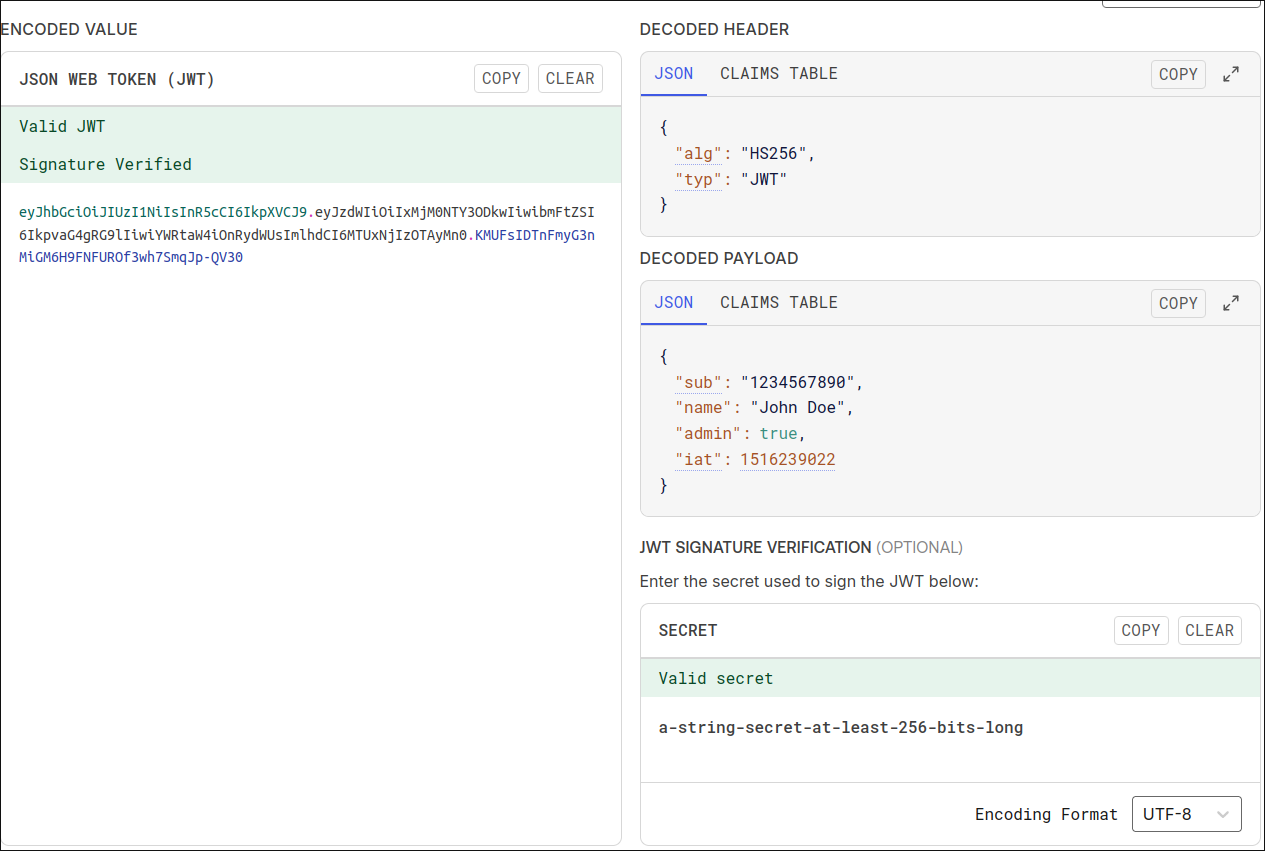
\includegraphics[width = 0.75\textwidth]{imgs/theoryJWT.png}
    \caption{Схема структуры JWT"=токена}
    \label{fig:JWT}
\end{figure}

% NOTE: Принцип использования JWT
Основной принцип использования JWT"=токенов заключается в том, что клиент получает токен после прохождения процесса аутентификации и передает его вместе с каждым запросом к защищенному ресурсу. Сервер в свою очередь, проверяет подлинность токена и разрешает доступ к ресурсу, если токен действителен. Таким образом, JWT"=токены позволяют реализовать механизм авторизации без необходимости хранения состояния на сервере. \cite{jwt2}

% NOTE: Стандарт RFC 7519
Стандарт RFC 7519 определяет несколько типов алгоритмов подписи, которые могут использоваться при создании JWT"=токенов. Некоторые из наиболее распространенных алгоритмов включают HMAC с использованием SHA"=256, RSA и ECDSA. Выбор алгоритма подписи зависит от требований безопасности и возможностей конкретной реализации.

Также стандарт определяет некоторые зарезервированные поля, которые могут использоваться в полезной нагрузке JWT"=токена. Некоторые из этих полей включают идентификатор пользователя (sub), дату истечения срока действия токена (exp), идентификатор клиента (aud).

\subsubsection{Хеширование паролей}

Безопасное хранение паролей пользователей является фундаментальной задачей при разработке систем аутентификации. Существует два способа хранения паролей в базеданных: в чистом виде и в виде зашифрованных значений. 

Хранение в чистом виде --- самый простой способ, при котором пароль хранится точно так, как его ввел пользователь. Это не безопасно, так как в случае утечки данных, злоумышленник может сразу использовать этот пароль.

Более распространённым и безопасным методом является хранение хэшированных паролей. Хэш"=функция --- это функция, которая принимает произвольное количество входных данных и выдает выходные данные фиксированного размера. При этом хэширование является односторонней операцией: восстановить исходный пароль из хэша практически невозможно.\cite{hashing1}

Использование хэш"=функций позволяет хранить не сами пароли, а их хэш"=суммы. В случае компрометации базы данных злоумышленник не сможет напрямую использовать хэши для доступа к аккаунтам. Для повышения безопасности к паролям добавляют случайные данные, называемые солью (salt), что предотвращает атаки с использованием радужных таблиц. Радужная таблица --- это предварительно вычисленный набор хэш"=значений. Эти таблицы позволяют злоумышленникам получать доступ к защищенным системам без подбора пароля.

 Хэш"=функция бывают обратимыми и необратимыми, однако для защиты паролей используют исключительно необратимые функции.

\textbf{Ключеве принципы хеширования паролей:}
\begin{itemize}
	\item{\textbf{Необратимость:} Хэш"=функции должны быть спроектированы так, чтобы обратное преобразование хэша в исходный пароль было невозможно}	
	\item{\textbf{Детерминированность:} Один и тот же пароль всегда генерирует идентичный хэш}
	\item{\textbf{ Соль (salt):} Случайные данные, добавляемые к паролю перед хэшированием для предотвращения атак радужными таблицами}
\end{itemize}



\section{Разработка серверной части приложения}

\subsection{Проектирование серверной части}

\subsubsection{Архитектура решения}

Архитектура серверной части проекта построена по принципу модульности, где каждый модуль (проект) отвечает за отдельный аспект системы:

\begin{itemize}
	\item{\textbf{Controllers}: Обрабатывает отправленные клиентом HTTP-запросы и возвращает ответы в формате JSON;}
	\item{\textbf{Services}: Реализует логику приложения;}
	\item{\textbf{Context}: Содержит настройки DbContext и инкапсулирует логику взаимодействия с базой данных (паттерн репозитории);}	
	\item{\textbf{Database}: Содержит сущности используемые для взаимодействия с базой данных;}
\end{itemize}

\subsubsection{Ролевая модель}
 
\begin{itemize}
	\item{Роль \guillemetleftстуеднт\guillemetright "--- пользователь, который может просматривать ленту запросов, записываться на запрос и отписываться от него. Также может просматривать и изменять данные своего аккаунта и получать запросы, на которые он записан.}
	\item{Роль \guillemetleftадминистратор\guillemetright "--- пользователь, который может все, что может \guillemetleftстуеднт\guillemetright, а также имеет доступ к CRUD операциям на запросы и пользователей. Также может отметить запрос как выполненный с начислением очков за него.}
	\item{Роль \guillemetleft Dev\guillemetright"--- пользователь, который может все, что может \guillemetleftстуеднт\guillemetright и \guillemetleftадминистратор\guillemetright , а также имеет доступ к повышению до администратора студента и понижению до студента администратора.}
\end{itemize}

\subsubsection{Спецификация API}

\begin{itemize}
	\item{/api/AdminRequest/ --- endpoint-ы для администраторов и Dev-ов по работе с запросами. Включает в себя CRUD для запросов, получение ленты запросов для администраторов и возможность отметить запрос как выполненный с начислением очков за него.}
	\item{/api/AdminUser/ --- endpoint-ы для администраторов Dev-ов по работе с пользователями. Включает в себя CRUD для пользователей.}
	\item{/api/Auth/ --- endpoint-ы для аутентификации пользователей. Включает в себя регистрацию, аутентификацию пользователей, обновление токена, отзыв токена и проверка своей роли (endpoint, возвращающий роль).}
	\item{/api/DevUser/ --- endpoint-ы для Dev-ов по работе с администраторами. Включает в себя возможность выдать роль администратора студенту и понизить администратора до студента.}
	\item{/api/StudentRequest/ --- endpoint-ы для студентов по работе с запросами. Включает в себя возможность получении ленты запросов для студента, записаться на запрос и отписаться с него.}
	\item{/api/User/ --- endpoint-ы для всех пользователей. Включает в себя получение информации о себе, изменение пароля и своих данных и получении информации о запросах, на которые он подписался.}
\end{itemize}

\subsection{Реализция серверной части}

\subsubsection{Структура решения (Сущности, сервисы, контроллеры)}

Пока не знаю как это вменяемо оформить.

\subsubsection{Реализация JWT}
% NOTE: JWT
Данная реализация JWT состоит из двух токенов:
\begin{enumerate}
	\item{\textbf{Access Token} --- короткоживущий (5 минут) токен, содержит основные claims (Id, имя пользователя, роль).}
	\item{\textbf{Refresh Token} --- долгоживущий (24 часа) токен, содержит аналогичные claims, но с дополнительным Jti (уникальный идентификатор).}
\end{enumerate}

Access Token используется для аутентификации пользователя и получения разрешения на доступ к защищенному ресурсу. Refresh Token используется для обновления Access Token в случае его устаревания. Так же для предотвращения использования украденных валидных Refresh Token, данный токен сохраняется в базе данных и удаляется при выходе пользователя из системы или повторном входе, что обеспечивает его недействительность и исключает возможность повторного применения после завершения сессии.

% NOTE: Генерация токенов:
\textbf{Генерация токенов:} По данным пользователя генерируются токены с учетом их времени жизни и соответствующими секретным ключам.
\begin{minted}{cs}
    private string GenerateAccessToken(User user, string secretKey)
    {
        var claims = GenerateClaimsAccess(user);
        var token = GenerateToken(claims, secretKey, accessTokenTime);
        return new JwtSecurityTokenHandler().WriteToken(token);
    }

    private string GenerateRefreshToken(User user, string secretKey)
    {
        var claims = GenerateClaimsRefresh(user);
        var token = GenerateToken(claims, secretKey + "sault", refreshTokenTime);
        return new JwtSecurityTokenHandler().WriteToken(token);
    }
\end{minted}
% \textbf{Подпись токенов:}
% \begin{enumerate}
% 	\item{Access Token подписывается с помощью ключа secretKey хранящегося в appsettings.json.}
% 	\item{Refresh Token подписывается с помощью того же ключа secretKey + строки "sault".}
% \end{enumerate}

% NOTE: Валидация Refresh Token 
\textbf{Валидация Refresh Token:} Если Refresh Token валиден, то возвращает Ok, если просрочен, то Ok с описанием, что время жизни токена истекло, иначе BadRequest с описанием, что токен невалидный.
\begin{minted}{cs}
    private BaseResponse<Tokens> ValidateRefreshToken(string token, string secretKey)
    {
        var tokenHandler = new JwtSecurityTokenHandler();
        var validationParameters = new TokenValidationParameters
        {
            ValidateIssuerSigningKey = true,
            IssuerSigningKey = new SymmetricSecurityKey(Encoding.ASCII.GetBytes(secretKey + "sault")),
            ValidateIssuer = false,
            ValidateAudience = false,
            ClockSkew = TimeSpan.Zero
        };
        try
        {
            // Проверка подписи JWT, если токен не верный будет исключение
            tokenHandler.ValidateToken(token, validationParameters, out _);
            return BaseResponse<Tokens>.Ok();
        }
        catch (SecurityTokenExpiredException ex)
        {
            return BaseResponse<Tokens>.Ok(description: "Token expired");
        }
        catch (SecurityTokenException ex)
        {
            return BaseResponse<Tokens>.BadRequest(description: "Tokens not valid");
        }
    }
\end{minted}

% NOTE: Обновление токенов:
\textbf{Обновление токенов:} Обновление токенов состоит из нескольких этапов:
\begin{itemize}
	\item{Проверка токена на валидность;}
\end{itemize}
\begin{minted}{cs}
    public async Task<IBaseResponse<Tokens>> RefreshToken(string oldRefreshToken, string secretKey)
    {
        BaseResponse<Tokens> response = ValidateRefreshToken(oldRefreshToken, secretKey);

        // Если oldRefreshToken невалидный
        if (response.StatusCode == StatusCodes.BadRequest)
        {
            return response;
        }
\end{minted}

\begin{itemize}
	\item{Перенос данных из Refresh Token в User для дальнейшего создания Access Token по этим данным:}
\end{itemize}
\begin{minted}{cs}
        var oldToken = new JwtSecurityTokenHandler().ReadJwtToken(oldRefreshToken);
        User user = new User();
        // Заполняем user на основе данных из oldRefreshToken
        user.Id = Convert.ToInt32(oldToken.Claims.First(
                    claim => claim.Type == JwtRegisteredClaimNames.Sub
                    ).Value);
        user.Name = Convert.ToString(oldToken.Claims.First(
                    claim => claim.Type == JwtRegisteredClaimNames.Name
                    ).Value);
        user.Role = Convert.ToString(oldToken.Claims.First(
                    claim => claim.Type == ClaimTypes.Role
                    ).Value);
\end{minted}

\begin{itemize}
	\item{Проверка на нахождение Refresh Token в базе данных (если его там нет, то считаем недействительным):}
\end{itemize}
\begin{minted}{cs}
        // Находим oldRefreshToken
        var oldRefreshDB = await _RefreshTokenRepository.FirstOrDefaultAsync(token => token.Token == oldRefreshToken);
        if (oldRefreshDB == null)
        {
            response = BaseResponse<Tokens>.NotFound();
            return response;
        }
\end{minted}

\begin{itemize}
	\item{Обновление Refresh Token, если токен не просрочен:}
\end{itemize}
\begin{minted}{cs}
        var oldTokenDB = new JwtSecurityTokenHandler().ReadJwtToken(oldRefreshDB.Token);

        // Оставляем старый refreshToken, или в случае просрока заменим далее
        string refreshToken = oldRefreshDB.Token;
        if (response.Description == "Token expired")
        {
            // Удаляем oldRefreshToken, если тот истек
            await _RefreshTokenRepository.Delete(oldRefreshDB);
            // Пересоздаем oldRefreshToken, если тот истек
            refreshToken = GenerateRefreshToken(user, secretKey);

            RefreshToken saveRefreshToken = new RefreshToken
            {
                Id = user.Id,
                Token = refreshToken
            };
            // Сохраняем новый refreshToken в бд
            await _RefreshTokenRepository.Create(saveRefreshToken);
        }
\end{minted}

\begin{itemize}
	\item{Создание Access Token по данным извлеченным из Refresh Token:}
\end{itemize}
\begin{minted}{cs}
        string accessToken = GenerateAccessToken(user, secretKey);
        response = BaseResponse<Tokens>.Ok(new Tokens
        {
            AccessToken = accessToken,
            RefreshToken = refreshToken
        });
        return response;
    }
\end{minted}

% NOTE: Удаление Refresh Token из бд: 
\textbf{Удаление Refresh Token из бд:} Удаление Refresh Token из базы данных по Id пользователя:
\begin{minted}{cs}
    public async Task<IBaseResponse> DeleteRefreshToken(int userId)
    {
        BaseResponse response;

        var refreshToken = await _RefreshTokenRepository.FirstOrDefaultAsync(token => token.Id == userId);

        if (refreshToken == null)
        {
            response = BaseResponse.NoContent();
            return response;
        }
        await _RefreshTokenRepository.Delete(refreshToken);

        response = BaseResponse.Ok();
        return response;
    }
\end{minted}

\subsubsection{Реализация ленты запросов, для администраторов и пользователей}

\textbf{Лента админов:}
\begin{minted}{cs}
        var respondedPeople = await _RespondedPeopleRepository.GetAll();

        List<PrivateRequest> requests;

        // Если есть откликнувшеся люди
        if (respondedPeople != null && respondedPeople.Count > 0)
        {
            // Ищем в БД
            requests = await _RequestRepository
                .GetQueryable()
                .Select(request => new PrivateRequest(request, respondedPeople))
                .ToListAsync();
        }
        else
        {
            // Ищем в БД
            requests = await _RequestRepository
                .GetQueryable()
                .Select(request => new PrivateRequest(request))
                .ToListAsync();
        }
\end{minted}

\textbf{Лента пользователей:}
\begin{minted}{cs}
        var respondedPeople = await _RespondedPeopleRepository.GetAll();

        List<PublicRequest> requests;

        // Если есть откликнувшеся люди
        if (respondedPeople != null && respondedPeople.Count > 0)
        {
            // Ищем в БД
            requests = await _RequestRepository
                .GetQueryable()
                .Select(request => new PublicRequest(request, respondedPeople))
                .ToListAsync();
        }
        else
        {
            // Ищем в БД
            requests = await _RequestRepository
                .GetQueryable()
                .Select(request => new PublicRequest(request))
                .ToListAsync();
        }
\end{minted}

\subsubsection{Реализация возможности записаться на запрос и отписаться с запроса}

\subsubsection{Реализация начисления очков за выполненный запрос}

\subsubsection{Реализация логирования изменений запроса администратором}

\subsubsection{Реализация повшения до администратора и понижения до пользователя}



\conclusion
В рамках проделанной работы была с помощью REST API на .NET реализована серверная часть системы, позволяющей преподавателям контролировать участие студентов в различных мероприятиях.

Система реализует ленту запросов, возможность записи и отписки с запроса. Была разработана система очков, получаемых студентов по результату участия в мероприятии, а также система логирования и ролевая модель, которая предоставляет возможность повышения и понижения участников.

Процесс аутентификации и авторизации был реализован с применением хэширования BCrypt, что делает эти процессы безопаснее.

% Отобразить все источники. Даже те, на которые нет ссылок.

\bibliographystyle{ugost2003}
\bibliography{thesis}

% Окончание основного документа и начало приложений Каждая последующая секция
% документа будет являться приложением
\appendix
\section{Полный код TokenServices}\label{app:TokenServices}
\begin{minted}{cs}
using System.IdentityModel.Tokens.Jwt;
using Microsoft.IdentityModel.Tokens;
using System.Security.Claims;
using System.Text;
using DataBase;
using Context;
namespace Services;

public class TokenServices : ITokenServices
{
    private readonly IRefreshTokenRepository _RefreshTokenRepository;
    private readonly int accessTokenTime = 5;
    private readonly int refreshTokenTime = 1440;

    public TokenServices(IRefreshTokenRepository refreshTokenRepository)
    {
        _RefreshTokenRepository = refreshTokenRepository;
    }

    public async Task<Tokens> GenerateJWTToken(User user, string secretKey)
    {
        Tokens jwtToken = new Tokens();

        string accessToken = GenerateAccessToken(user, secretKey);
        string refreshToken = GenerateRefreshToken(user, secretKey);

        jwtToken.AccessToken = accessToken;
        jwtToken.RefreshToken = refreshToken;

        RefreshToken saveRefreshToken = new RefreshToken();
        saveRefreshToken.Id = user.Id;
        saveRefreshToken.Token = refreshToken;

        // Находим oldRefreshToken
        var oldRefreshDB = await _RefreshTokenRepository.FirstOrDefaultAsync(token => token.Id == saveRefreshToken.Id);
        // Удаляем oldRefreshToken, если тот есть
        if (oldRefreshDB != null)
        {
            await _RefreshTokenRepository.Delete(oldRefreshDB);

        }
        await _RefreshTokenRepository.Create(saveRefreshToken);

        return jwtToken;
    }

    public async Task<IBaseResponse<Tokens>> RefreshToken(string oldRefreshToken, string secretKey)
    {
        BaseResponse<Tokens> response = ValidateRefreshToken(oldRefreshToken, secretKey);

        // Если oldRefreshToken невалидный
        if (response.StatusCode == StatusCodes.BadRequest)
        {
            return response;
        }

        var oldToken = new JwtSecurityTokenHandler().ReadJwtToken(oldRefreshToken);
        User user = new User();
        // Заполняем user на основе данных из oldRefreshToken
        user.Id = Convert.ToInt32(oldToken.Claims.First(
                    claim => claim.Type == JwtRegisteredClaimNames.Sub
                    ).Value);
        user.Name = Convert.ToString(oldToken.Claims.First(
                    claim => claim.Type == JwtRegisteredClaimNames.Name
                    ).Value);
        user.Role = Convert.ToString(oldToken.Claims.First(
                    claim => claim.Type == ClaimTypes.Role
                    ).Value);

        // Находим oldRefreshToken
        var oldRefreshDB = await _RefreshTokenRepository.FirstOrDefaultAsync(token => token.Token == oldRefreshToken);

        if (oldRefreshDB == null)
        {
            response = BaseResponse<Tokens>.NotFound();
            return response;
        }

        var oldTokenDB = new JwtSecurityTokenHandler().ReadJwtToken(oldRefreshDB.Token);


        // Оставляем старый refreshToken, или в случае просрока заменим далее
        string refreshToken = oldRefreshDB.Token;
        if (response.Description == "Token expired")
        {
            // Удаляем oldRefreshToken, если тот истек
            await _RefreshTokenRepository.Delete(oldRefreshDB);
            // Пересоздаем oldRefreshToken, если тот истек
            refreshToken = GenerateRefreshToken(user, secretKey);

            RefreshToken saveRefreshToken = new RefreshToken
            {
                Id = user.Id,
                Token = refreshToken
            };
            // Сохраняем новый refreshToken в бд
            await _RefreshTokenRepository.Create(saveRefreshToken);
        }

        string accessToken = GenerateAccessToken(user, secretKey);
        response = BaseResponse<Tokens>.Ok(new Tokens
        {
            AccessToken = accessToken,
            RefreshToken = refreshToken
        });
        return response;
    }

    public async Task<IBaseResponse> DeleteRefreshToken(int userId)
    {
        BaseResponse response;

        var refreshToken = await _RefreshTokenRepository.FirstOrDefaultAsync(token => token.Id == userId);

        if (refreshToken == null)
        {
            response = BaseResponse.NoContent();
            return response;
        }
        await _RefreshTokenRepository.Delete(refreshToken);

        response = BaseResponse.Ok();
        return response;
    }

    private string GenerateAccessToken(User user, string secretKey)
    {
        var claims = GenerateClaimsAccess(user);
        var token = GenerateToken(claims, secretKey, accessTokenTime);
        return new JwtSecurityTokenHandler().WriteToken(token);
    }

    private string GenerateRefreshToken(User user, string secretKey)
    {
        var claims = GenerateClaimsRefresh(user);
        var token = GenerateToken(claims, secretKey + "sault", refreshTokenTime);
        return new JwtSecurityTokenHandler().WriteToken(token);
    }

    private JwtSecurityToken GenerateToken(Claim[] claims, string secretKey, int time)
    {
        var key = new SymmetricSecurityKey(Encoding.UTF8.GetBytes(secretKey));
        var creds = new SigningCredentials(key, SecurityAlgorithms.HmacSha256);

        var token = new JwtSecurityToken(
                issuer: "axecac-kek.ru",
                audience: "axecac-kek.ru",
                claims: claims,
                expires: DateTime.Now.AddMinutes(time),
                signingCredentials: creds);

        return token;
    }

    private Claim[] GenerateClaimsAccess(User user)
    {
        var claims = new[]
        {
            new Claim(JwtRegisteredClaimNames.Name, user.Name),
            new Claim(JwtRegisteredClaimNames.Sub, user.Id.ToString()),
            new Claim(ClaimTypes.Role, user.Role),
        };
        return claims;
    }

    private Claim[] GenerateClaimsRefresh(User user)
    {
        var claims = new[]
        {
            new Claim(JwtRegisteredClaimNames.Name, user.Name),
            new Claim(JwtRegisteredClaimNames.Sub, user.Id.ToString()),
            new Claim(JwtRegisteredClaimNames.Jti, Guid.NewGuid().ToString()),
            new Claim(ClaimTypes.Role, user.Role),
        };
        return claims;
    }

    private BaseResponse<Tokens> ValidateRefreshToken(string token, string secretKey)
    {
        var tokenHandler = new JwtSecurityTokenHandler();
        var validationParameters = new TokenValidationParameters
        {
            ValidateIssuerSigningKey = true,
            IssuerSigningKey = new SymmetricSecurityKey(Encoding.ASCII.GetBytes(secretKey + "sault")),
            ValidateIssuer = false,
            ValidateAudience = false,
            ClockSkew = TimeSpan.Zero
        };
        try
        {
            // Проверка подписи JWT, если токен не верный будет исключение
            tokenHandler.ValidateToken(token, validationParameters, out _);
            return BaseResponse<Tokens>.Ok();
        }
        catch (SecurityTokenExpiredException ex)
        {
            return BaseResponse<Tokens>.Ok(description: "Token expired");
        }
        catch (SecurityTokenException ex)
        {
            return BaseResponse<Tokens>.BadRequest(description: "Tokens not valid");
        }
    }
}
\end{minted}


\section{Архив с окончательным вариантом решения}\label{app:Others}

В приложенном флеш накопителе, для ознакомления, содержатся файлы и код решения и файл данной работы в pdf формате.


\end{document}
